\documentclass[11pt]{article}

\newif\ifBenchTikzExternalize
\BenchTikzExternalizefalse
\InputIfFileExists{bench-config.tex}{}{}

\newcommand{\benchtexttoken}{ALPHA}
\newcommand{\benchfiguretoken}{1.00}
\newcommand{\benchpreambletoken}{P0}

\usepackage{amsmath}
\usepackage{amssymb}
\usepackage{booktabs}
\usepackage{hyperref}
\usepackage{tikz}

\title{W1 Text-Math Workload}
\author{FastXeBench}
\date{}

\begin{document}
\maketitle

\section{Motivation}
The benchmark token is \benchtexttoken. This workload mixes prose, inline math, displayed equations, cross-references, bibliography activity, and a lightweight figure \cite{refalpha}.

\section{Model}
Consider the edit-to-PDF objective
\begin{equation}
\label{eq:objective}
J(\theta) = \sum_{i=1}^{n} \left(y_i - \hat{y}_i(\theta)\right)^2 + \lambda \lVert \theta \rVert_2^2 .
\end{equation}
Equation~\eqref{eq:objective} is referenced twice so that reruns still exercise the auxiliary-file path.

\section{Result}
Table~\ref{tab:summary} and Figure~\ref{fig:triangle} are intentionally simple but stable.

\begin{table}[h]
\centering
\begin{tabular}{@{}lrr@{}}
\toprule
Metric & Cold build & Incremental build \\
\midrule
Median latency & 5.2 & 1.7 \\
IQR & 0.8 & 0.4 \\
\bottomrule
\end{tabular}
\caption{Placeholder values for a stable text-math workload.}
\label{tab:summary}
\end{table}

\begin{figure}[h]
\centering
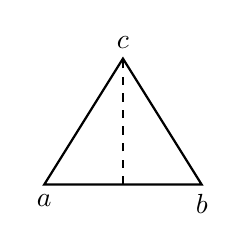
\begin{tikzpicture}[scale=\benchfiguretoken]
  \draw[thick] (0,0) -- (2,0) -- (1,1.6) -- cycle;
  \draw[dashed] (1,0) -- (1,1.6);
  \node[below] at (0,0) {$a$};
  \node[below] at (2,0) {$b$};
  \node[above] at (1,1.6) {$c$};
\end{tikzpicture}
\caption{A figure whose scale changes under the figure-edit scenario.}
\label{fig:triangle}
\end{figure}

As shown in Figure~\ref{fig:triangle}, the body-level edit and figure-level edit are independent in this synthetic case.

\bibliographystyle{plain}
\bibliography{refs}

\end{document}
